\clearpage
\section{More Background on Maintaining Resharding Scripts}
\label{sec:reshard_scripts}

\begin{figure}[!t]
  \centering
  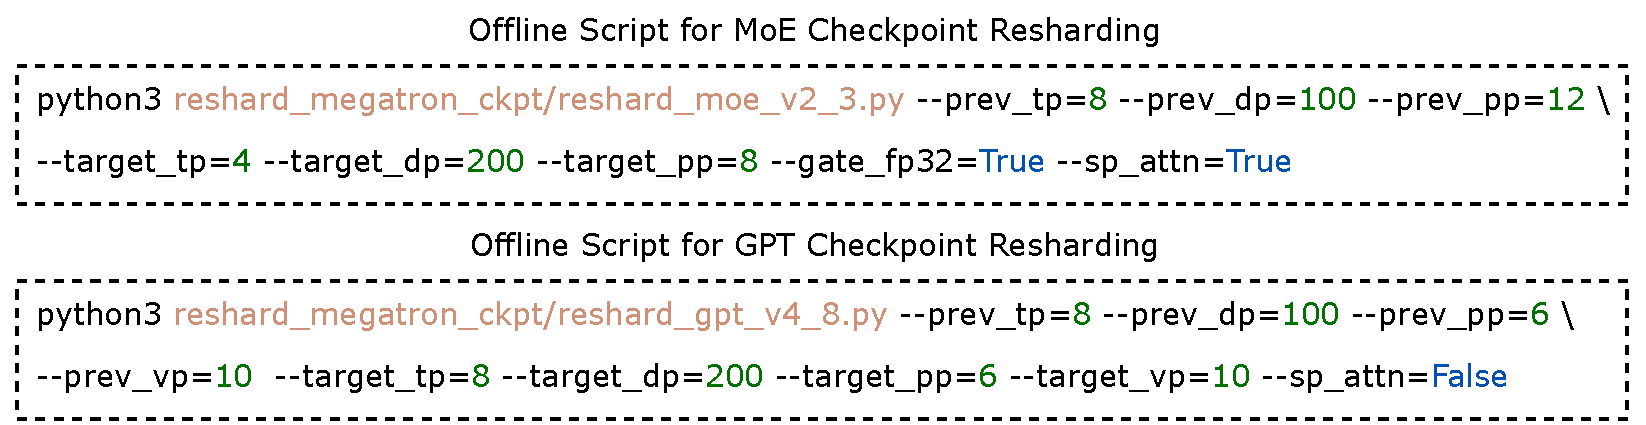
\includegraphics[width=\linewidth]{figures/scripts_example.pdf}
  \caption{
  Examples of running offline scripts for checkpoint resharding.
  }
  \label{fig:script_example}
\end{figure}

Examples of offline resharding with customized scripts are given in Fig.~\ref{fig:script_example}.
% \textit{First}, %the development of 
Customizing offline scripts %lacks extensibility and 
is labor-intensive. %significant maintenance overhead.
For GPU state resharding, the offline scripts must cover all different components in the LFM and its optimizer and cater to the diverse behavior of each component under different parallelism strategies.
For example, with Tensor Parallelism (TP), %designed for LLM training~\cite{megatron}, two 
GEMM operators in attention and MLP blocks are sharded along different dimensions, while other operators like LayerNorm~\cite{layernorm} are replicated across GPUs.
When hybrid 3D parallelism~\cite{megatron-lm2} is adopted, %instead of directly sharded along the original dimension, 
TP-sharded tensors of one layer (module) in the distributed optimizer are first flattened and then merged before being sharded according to the designated Data Parallelism (DP) degree.
Offline scripts must implement resharding logic that is tightly coupled with combinations of model (optimizer) components and parallelism strategies. %to meet various requirements.
Additionally, special algorithmic optimization techniques such as GQA~\cite{gqa} and MLA~\cite{deepseek} change the tensor layout of certain operators %in these components 
(e.g., the query-key-value projection GEMM operator in the attention block), necessitating corresponding resharding support.
% (\textbf{@yiyao: discuss drawbacks of dataloader offline resharding if there exists any ones.})
To handle various cases in our production environment,
% xxx \cwu{give the number} versions of resharding scripts are tailored, %for specific tasks.
our largest script even includes 3193 lines of Python code.
This complexity results in significant engineering efforts for both development and maintenance. 


%\section{Dataloader}

%\subsection{Dataloader and Extra State Representation}
%\label{sec:loader_extra}
%The dataloader states can be categorized into
%two types: \textit{replicated} states and \textit{sharded} states. Replicated states %include the number of data reading workers, paths to source datasets, and sampling %ratios, and are identical across all I/O workers (subprocesses) in different ranks.
%% \cwu{clarify what an I/O worker is}
%Sharded states are unique to each I/O worker, including the token buffer %(as %described in Sec. 2) 
%and data retrieval offsets for different data sources. % Our system, \
%In \sys{}, %employs an efficient storage strategy: 
%sharded states are saved in individual files, while replicated states are saved only %by the I/O worker in rank 0. This %approach offers two key advantages: 
%reduces overall %checkpoint 
%size of dataloader states to be saved and facilitates dataloader resharding when %parallelism configurations change since the separation of data states into distinct %files simplifies %the process of 
%states merging and redistributing according to the new parallelism. For other extra %states such as the RNG state, we pack and 
%serialize them into one compact byte object before dumping them into storage.

%\subsection{Dataloader Resharding}
%\label{sec:dataloader_reshard}
%\begin{figure}[!t]
%  \centering
%  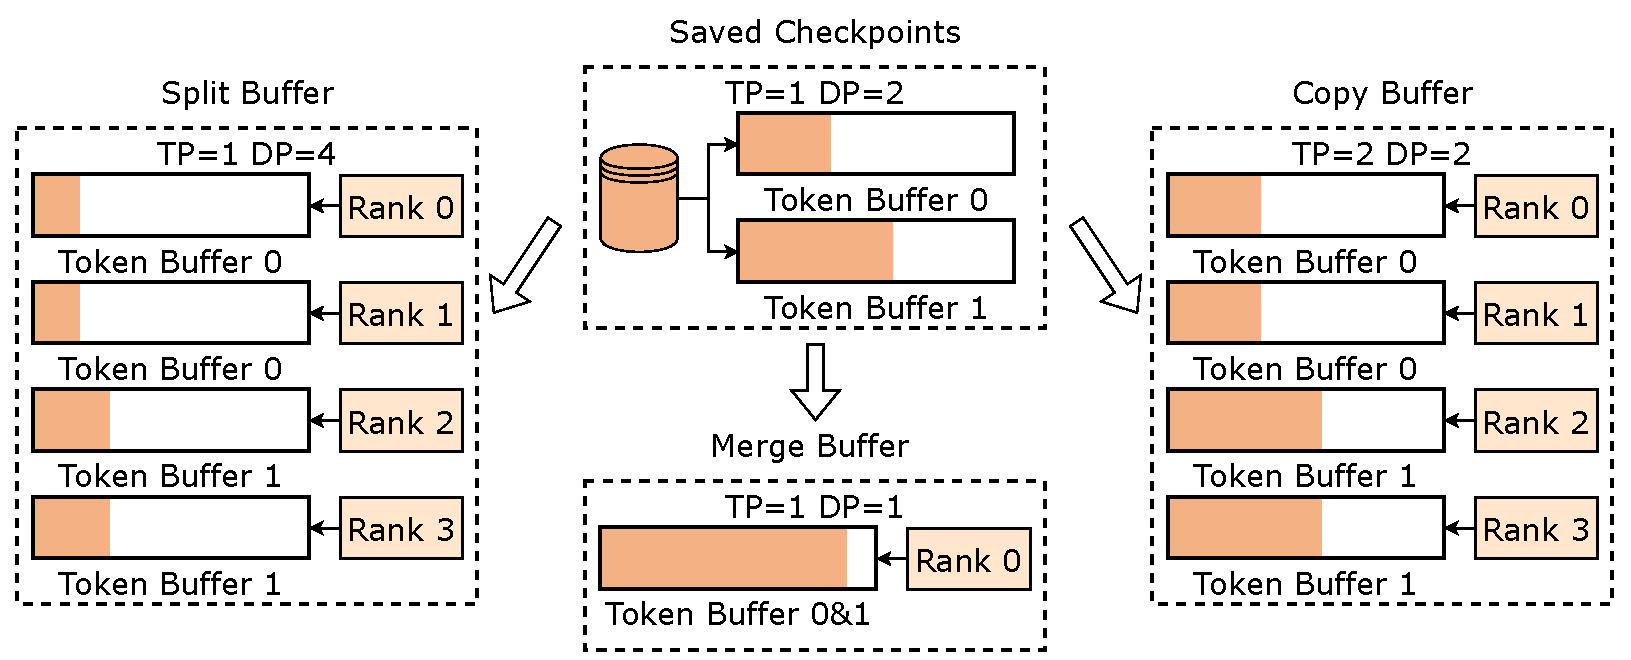
\includegraphics[width=\linewidth]{figures/loader_reshard_examples.pdf}
%  \caption{
%  Examples of dataloader resharding.
%  Unique items such as cumulative token buffers are resharded according to the changes %of 
%  parallelism configurations.
%  We do not depict data retrieval offsets for clarity of the figure.
%  }
%  \label{fig:loader_reshard_example}
%\end{figure}

% \yhpeng{we need to find a better place to discuss dataloader resharding.}
%The illustration of dataloader resharding is depicted in %Fig.~\ref{fig:loader_reshard_example}. When parallelism configuration changes, for the %dataloader checkpoints, common items in the dataloader checkpoints can be loaded %directly, whereas unique items such as accumulative token buffers and data retrieval %offsets require resharding. Specifically, when the DP degree size remains constant %while other parallel degrees are altered (TP degree changes in the example of %Fig.~\ref{fig:loader_reshard_example}), the token buffers should be copied to the %destination workers for bitwise-correct resuming. when there is a change in the DP %degree size, the token buffers must be either split or merged accordingly to ensure %that the resumed dataloaders do not discard cached data and do not retrain data that %has already been sampled and fed. Thanks to the split storage strategy designed for %the dataloader module, \sys{} can precisely identify the unique items that require %resharding and process them efficiently.

%\section{Other Important Optimizations}
%\subsection{High Performance Read/Write}\label{sec:io_parallel}
%% \yhpeng{TODO: Add numbers in the sentences to illustrate the performance before and %after optimization and polish the writing.}
%% \zmf{polished at 09/17 10:33 GMT+8}
%We optimize read and write throughput of checkpointing by tailoring our implementation %to optimal I/O %patterns 
%usage of commonly used storage backends. For example, while HDFS is not primarily %designed for random data access, it does offer some random read capabilities via its %SDK, allowing applications to access specific file offsets and retrieve data from %those positions. We leverage this feature %we have enhanced our C++ HDFS SDK to %support 
%and enable multi-threaded reading of a single file, significantly accelerating the %download speed of checkpoint files from HDFS. In our production platform, single-file %read speed has improved from 400 MB/s to 2-3 GB/s, all tested on H800 servers equipped %with over 100 CPU cores, TB-level memory, and a 200Gbps NIC.

%For file writing, HDFS's append-only write %mechanism
%makes it impractical to split a single file into multiple parts based on offsets for %multi-threaded writing. To overcome this limitation, we %introduced a workaround in %the HDFS SDK that 
%split the target file into several sub-files of fixed size and concurrently write %%These sub-files are then concurrently written 
%them into HDFS using multi-threading. After the upload is complete, we perform %metadata-level concatenation to seamlessly merge the sub-files back into a single %entity, ensuring integrity of the stored data blocks. %Under ideal network conditions, %free from cross-datacenter issues or network congestion, 
%Without network congestion, %the end-to-end 
%single-file upload speed can reach %up to 
%3 GB/s, far exceeding the average read/write throughput of a single HDFS client (under %100 MB/s%(according to the open-source benchmarks for HDD HDFS clusters
%~\cite{shvachko2010hdfs}). %It is important to note that the actual performance of HDFS can be significantly influenced by the hardware equipment of both the client and HDFS server.

%\yhpeng{is there any baseline e.g., open-source HDFS's single file write performance? If so, add the baseline performance} \zmf{added a comparison with open benchmark on HDD HDFS. HDFS performance metrics are highly dependent on the hardware environment, so open-source HDFS benchmarks have limited reference value and should only be used for informal comparisons.}

%We have optimized checkpointing read and write throughput performance for our commonly used storage backends. Take HDFS as an example, although HDFS is not primarily engineered for random data access, it does provide a degree of random read functionality through its SDK.
%This allows applications to navigate to specific offsets within a file and initiate data retrieval from those points. Leveraging this feature, we have enhanced our C++ HDFS SDK to include multi-threading reading of a single file, significantly accelerating the download speed of checkpoint files from HDFS. In our production environment, the measured single-file read performance has been improved from 200 MiB/s to 2-3 GiB/s.

%For file writing, due to the append-only write mechanism inherent in HDFS, it is impractical to directly split a single file into multiple parts based on offsets to enable multi-threaded writing. To circumvent this limitation, we implement a workaround method in which the HDFS SDK splits the file intended for writing into several sub-files of a fixed size. These sub-files are then written into HDFS using the multi-threading technique.
%After uploading, we facilitate a concatenate operation at the metadata level.
%This operation seamlessly merges the sub-files back into a single file, ensuring that the integrity of the stored data blocks remains intact.
%In an ideal scenario without cross-datacenter issues or network congestion, the end-to-end single-file upload performance can also reach up to 3 GiB/s.


\section{Efficient Integrity Guarantee}
\label{sec:barrier_check}

% Guaranteeing the integrity of checkpoints is also important in large-scale training.
% As massive checkpoint data produced by thousands of training workers are periodically moved across various storage media (GPU memory, CPU memory, local disks, HDFS, and NAS), errors occurring in any worker during this process can incur incompleteness of the distributed checkpoints. 
A complete checkpoint consists of multiple files stored by different workers. The failure of any single worker can corrupt the entire checkpoint.
To prevent such issues, a barrier mechanism is essential to achieve atomic save/load operations among all training workers. 
% \yhpeng{not sure if we need to mention ckpt integrity here. I think this paragraph can be deleted.}

Checkpointing modules in training frameworks like Megatron-LM~\cite{megatron} rely on the \texttt{barrier} function in \texttt{torch.distributed} to perform integrity checks.
This approach synchronizes training workers to ensure that all checkpoint saving/loading operations are finished.
% \cwu{how is it related to ensuring integrity in case of  worker failure}
% albeit at the cost of blocking training.
We observed that when scaling training to involving approximately 10,000 GPUs, this behavior results in stalls of about 20 seconds each time.
To address this inefficiency, we re-implement the \texttt{barrier} function using the aforementioned method (gRPC with tree-based communication topology) 
% \cwu{what the aforementioned method is?} 
and conduct the integrity checks asynchronously, 
% \cwu{clarify what integrity checks do exactly},
effectively eliminating the blocking time. We also incorporate upload/download retry mechanisms in \sys{}'s I/O workers
% \cwu{who retry what?}
and integrate failure logging, which records the exact stage of failure within the checkpoint saving/loading pipelines in workers who fail to complete checkpointing tasks.
% \cwu{briefly tell how the failure logging works}
% to identify workers that fail to complete checkpointing tasks, aiding further diagnosis \cwu{diagnosis for what? how is it related to checkpointing integrity?}.

\section{Average ETTR Calculation}\label{sec:ettr_cal}
Failures that happened during training introduce progress loss and the last checkpoint loading overhead.
Assume failures are evenly distributed within one checkpoint interval~\cite{gemini-sys}, the best case is that a failure occurs just after the completion of a checkpoint end-to-end saving procedure whereas the worst case is just before that.
Given the per iteration training time $T_{iter}$, checkpoint interval $N$, end-to-end checkpoint saving time $T_{save}$ and loading (resharding) time $T_{load}$, we derive the average wasted time $T_{wasted}$ as:
\begin{equation}
    T_{wasted} = T_{save} + T_{load} + \frac{N \cdot T_{iter}}{2}
\end{equation}
Therefore, the average ETTR is:
\begin{equation}
    ETTR = 1 - \frac{T_{wasted}}{T_{save} + T_{load} + N\cdot T_{iter}}
\end{equation}

The end-to-end ETTR results presented in Table~\ref{tab:io_compare} are averaged across standard loading and resharding settings.



\section{Checkpointing Overhead Breakdown}
\label{sec:save_breakdown}
We break down the end-to-end checkpoint saving time ($\mathbf{T_{save}}$) for rank 0 by dividing it into several phases and investigating the overhead of each part.
The results are depicted in Table~\ref{tab:save_breakdown}, where $\mathbf{T_{Plan}^{First}}$ denotes the initial planning cost while $\mathbf{T_{Plan}^{Cache}}$ refers to the overhead when using the plan and metadata cache for subsequent checkpointing operations.
Costs of other phases are averaged over various checkpointing steps.
We find that the communication overhead of planning increases as training scales up, leading to significant stalls. 
Thanks to the caching strategy (Sec.~\ref{sec:opt_plan}), it becomes a one-time expense for each (resumed) training session.
In addition, the adoption of the pinned memory CPU pool renders the blocking time of D2H almost negligible, while our asynchronous engine pipeline overlaps the execution time of serialization, shared memory dumping, and HDFS uploading, diminishing the end-to-end time.
Furthermore, the load-balancing mechanism exploits the capabilities for parallel uploading within each DP group and achieves more performance gains at larger training scales (e.g., the uploading speed of model states with 4800 GPUs is 3.03$\times$ faster than that with 2400 GPUs). 

\begin{table*}[!t]
\caption{Detailed overhead breakdown of the checkpoint saving procedure for rank 0.}
\label{tab:save_breakdown}
\begin{small}
\resizebox{\linewidth}{!}{
\begin{tabular}{c|cc|ccccccc}
    \toprule
    \textbf{Model and Framework} & \textbf{Source \#GPUs} & \textbf{State} & $\mathbf{T_{Plan}^{First}}$ \textbf{(s)} & $\mathbf{T_{Plan}^{Cache}}$ \textbf{(s)} & $\mathbf{T_{D2H}}$ \textbf{(s)} & $\mathbf{T_{Serialize}}$ \textbf{(s)} & $\mathbf{T_{Dump}}$ \textbf{(s)} & $\mathbf{T_{Upload}}$ \textbf{(s)}\\
    \midrule
     \multirow{2}{*}{vDiT 4B} & \multirow{2}{*}{32} & Model & 0.05 & 0.00 & 0.15 & 0.52 & 0.50 & 11.04\\
     & & Optimizer & 0.65 & 0.00 & 0.37 & 0.93 & 1.03 & 14.60 \\
     \cline{2-9}
     \multirow{2}{*}{FSDP} & \multirow{2}{*}{128} & Model & 0.35 & 0.00 & 0.06 & 0.29 & 0.12 & 10.57 \\
     & & Optimizer & 0.89 & 0.00 & 0.06 & 0.29 & 0.26 & 9.85 \\
     \midrule
     \multirow{2}{*}{tGPT 70B} & \multirow{2}{*}{2400} & Model & 8.39 & 0.00 & 0.08 & 1.93 & 0.48 & 6.67\\
     & & Optimizer & 5.02 & 0.00 & 0.17 & 2.00 & 2.23 & 2.30 \\
     \cline{2-9}
     \multirow{2}{*}{Megatron-LM} & \multirow{2}{*}{4800}  & Model & 17.09 & 0.00 & 0.08 & 1.95 & 0.47 & 2.20 \\
     &  & Optimizer & 6.46 & 0.00 & 0.03 & 1.69 & 0.35 & 1.67 \\
    \bottomrule
\end{tabular}}
\end{small}
\end{table*}



\section{More Resharding Correctness Experiments}
\label{sec:exp_full_correct}

\begin{figure}[!t]
    \centering    
     \begin{subfigure}[b]{0.49\linewidth}
         \centering
         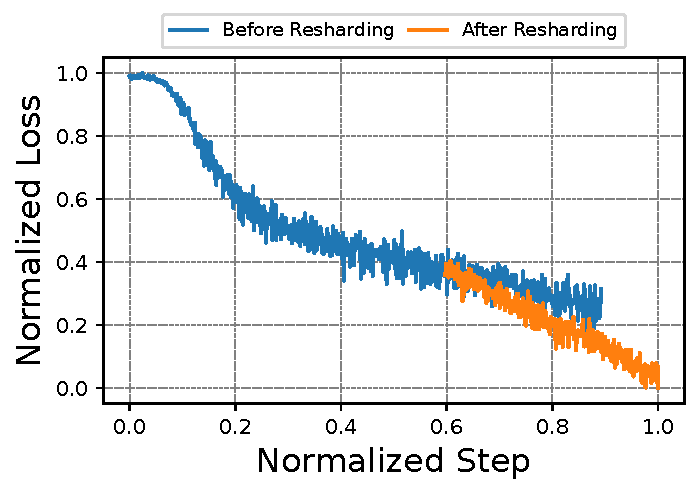
\includegraphics[width=\linewidth]{figures/dp_resharding.pdf}
         \caption{DP resharding from TP=1, DP=4, PP=4 to TP=1, DP=8, PP=4.}
         \label{fig:dp_resharding}
     \end{subfigure}
     \hfill
     \begin{subfigure}[b]{0.49\linewidth}
         \centering
         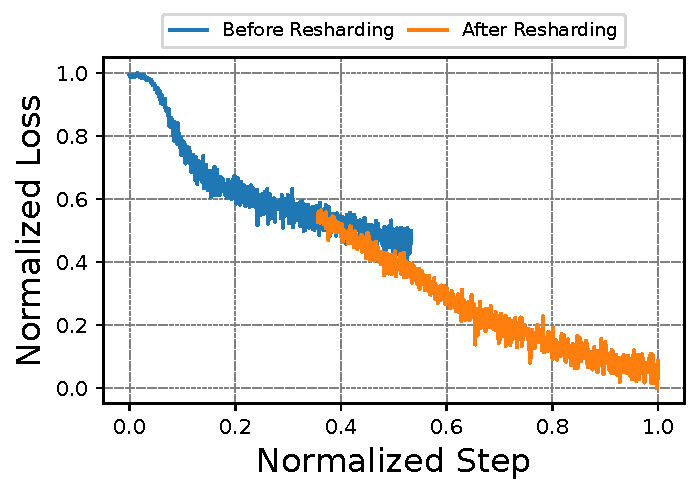
\includegraphics[width=\linewidth]{figures/hp_resharding.pdf}
         \caption{Hybrid resharding from TP=1, DP=4, PP=4 to TP=2, DP=8, PP=2.}
         \label{fig:hp_resharding}
     \end{subfigure}
     \caption{Resharding correctness verification.}
      \label{fig:reshard_full_correct}
\end{figure}

\begin{figure}[!t]
  \centering
  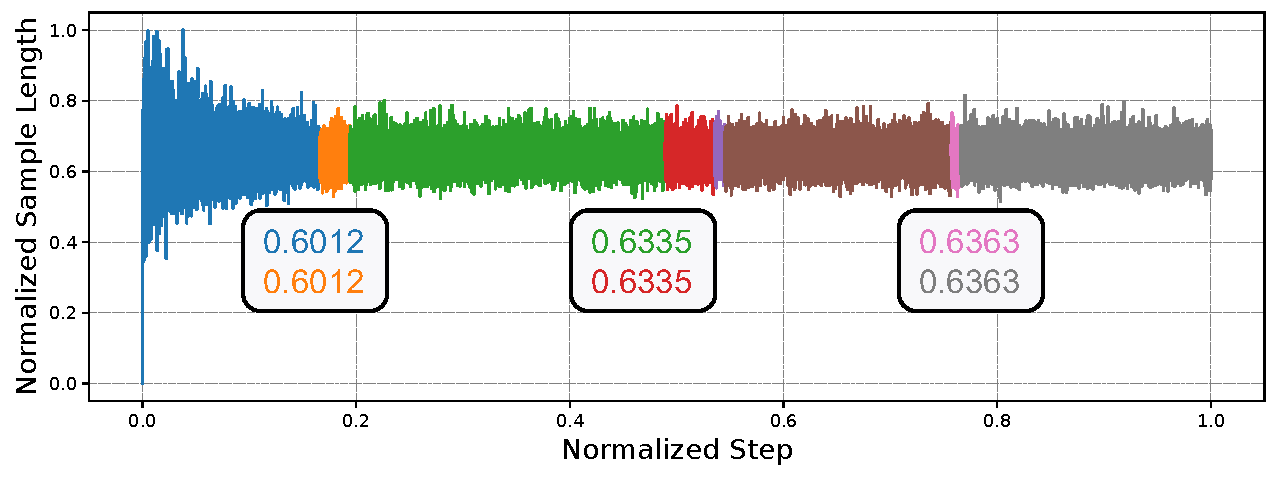
\includegraphics[width=\linewidth]{figures/online_resume_length.pdf}
  \caption{
  The normalized sample length curves of the dataloader with multiple training restarts. 
  }
  \label{fig:loader_resume}
\end{figure}


The normalized loss curves for DP and hybrid resharding correctness are shown in Fig.~\ref{fig:reshard_full_correct}.
In the case of DP and hybrid resharding, since we also increase the global batch size, the loss curve after resharding declines more rapidly.

We further show that \sys{} can achieve bit-wise correct resuming for dataloader states.
Since the RNG state is fixed, correct resumptions should yield the same data sampling trajectory.
Therefore, we use the normalized data sample length curve (Fig.~\ref{fig:loader_resume}) for evaluation.
As highlighted, the normalized data sample length before and after restarts is identical.

\section{Related Work}
\label{sec:related_work}

%\begin{table*}[!t]
%\caption{Comparison of existing checkpointing systems.
%}
%\label{tab:baseline_compare}
%\resizebox{\linewidth}{!}{
%\begin{tabular}{ccccc}
%    \toprule
%    \textbf{System} & \textbf{Multi-Parallel Strategy} & \textbf{Multi-Framework} & \textbf{Online Resharding} & \textbf{Scalabilty} \\
%    \midrule
%     CheckFreq~\cite{checkfreq} & \without & \without & \without & \without \\
%     Check-N-Run~\cite{check-n-run} & \without & \without & \without & \with \\
%     Gemini~\cite{gemini-sys} & \without & \without & \without & \without \\
%     JIT Checkpointing~\cite{jit-check} & \without & \without & \without & \without \\
%     DCP~\cite{torch-dcp} & \without & \without & \with & \without \\
%     MCP~\cite{megatron-dcp} & \without & \without & \with & \without \\
%     \sys{} & \with & \with & \with & \with \\
%    \bottomrule
%\end{tabular}}
%\end{table*}
%\vspace{-3mm}
%We summarize the features of different checkpointing systems in Table~\ref{tab:baseline_compare} and give a detailed discussion about existing works as follows: %\yhpeng{what does general purpose in the table mean? Consider using another term, e.g., large-scale?} 
% \yhpeng{The table can be deleted.}

% \yhpeng{we need more references here}

\noindent \textbf{Checkpointing frameworks.} %\yhpeng{discuss how PyTorch does checkpointing before DCP; also briefly discuss DeepSpeed UCP saying it is offline script}
Some industrial initiatives focus on developing checkpointing systems for deep learning. Prior to DCP~\cite{torch-dcp}, PyTorch provided \texttt{torch.save} and \texttt{torch.load} APIs for local checkpoint management, without native resharding support. DCP~\cite{torch-dcp} introduced resharding capabilities for FSDP but lacks support for %hybrid
parallelism strategies such as TP and PP. DeepSpeed-UCP~\cite{deepspeed-ucp} provides a unified format for DeepSpeed checkpoints and offers resharding capabilities through offline scripts. Megatron MCP~\cite{megatron-dcp} builds upon the workflow of DCP~\cite{torch-dcp} and extends storage options to formats like Zarr~\cite{Zarr}. %However, 
All these frameworks provide limited support for various parallelism strategies and training frameworks, %(e.g., MCP only works for Megatron-LM~\cite{megatron}). 
% \zmf{the "limited support" and the reasons why "they cannot fulfill the demand" can be elaborated more in details.}
% Therefore, they cannot meet the multi-framework support requirement.
% Moreover, both DCP and MCP struggle with complex, irregular-sharded tensors in hybrid parallel training (see details in Sec.~\ref{sec:representation}), hindering their applicability in general scenarios.
%Additionally, when deployed for
and their I/O performance does not scale well in large-scale training.  %remains sub-optimal, and scalability becomes an issue. 
% Additionally, the centralized communication pattern used for process orchestration (See Sec.~\ref{sec:workflow}) in DCP~\cite{torch-dcp} and MCP~\cite{megatron-dcp} also presents potential stability risks. \sys{} address these limitations, enabling flexible multi-framework checkpointing support, as well as guaranteeing stability and efficiency at scale.

\noindent \textbf{Checkpointing optimizations.} Several %previous
works \cite{projectadam, deepfreeze} %\yhpeng{add citations of 2-3 papers here} 
 investigated reducing checkpointing costs from different perspectives.
Check-N-Run~\cite{check-n-run}, designed for recommendation models, employs differential checkpointing to store only the modified portions of the model, alongside quantization %techniques
to reduce checkpoint size. % However, differential checkpointing is not directly applicable to the Pre-Training of LLMs, as LLMs typically exhibit dense updating patterns. The quantization technique is beyond the scope of this work, given that lossless checkpoints are imperative in our production settings.
CheckFreq~\cite{checkfreq} pipelines snapshot and save operations with computation to minimize checkpoint stalls and introduces an online algorithm for tuning checkpoint frequency to further lower costs. 
Gemini~\cite{gemini-sys} advocates for in-memory checkpointing with inter-machine backup for fast recovery, interleaving checkpoint communication with training traffic to enable frequent checkpoints per iteration.
JIT-Checkpointing~\cite{jit-check} adopts just-in-time checkpointing for low-cost error recovery.
%\mingji{Both CheckFreq~\cite{checkfreq} and Gemini~\cite{gemini-sys} focus on checkpoint efficiency during training.} 
%However, Gemini~\cite{gemini-sys}'s in-memory checkpointing solution demonstrates vulnerabilities in real-world large-scale GPU clusters, where multiple machines within the same backup group can experience simultaneous failures, leading to unacceptable catastrophic state loss. Other checkpointing techniques like Just-In-Time checkpointing  also suffer from the same reliability problem as Gemini~\cite{gemini-sys}. %\yhpeng{do not argue in this way regarding to Gemini and JIT. Maybe we can say these techniques are complementary and we can also use these techniques for better failure recovery} 
In industrial use cases, it is crucial to store checkpoints in separate persistent storage for various tasks such as auto-evaluation~\cite{characterization}, hyper-parameter tuning, and model debugging.
ServerlessLLM~\cite{serverlessllm} focuses on the demand for loading optimizations which is critical in serverless inference scenarios.
It proposes a chunk-based, multi-tier loading pipeline to accelerate checkpoint loading.
%Regarding the latter, after making configuration adjustments, the checkpoint with the highest evaluation scores is likely to be selected as the new starting point. 
Unlike existing solutions, \sys{} champions both optimized I/O performance and flexible load-time checkpoint resharding, supporting general LFM development.

\noindent \textbf{Checkpoint representation.}
PyTorch's \texttt{torch.save/load} functionality relies on \texttt{pickle} for serialization and deserialization.
This format lacks crucial tensor shard metadata, such as global shape information, precluding automatic resharding.
DCP \cite{torch-dcp} addresses this limitation by introducing a disaggregated format that separates metadata from tensor data. This metadata, which includes global shape and offset details, enables automatic resharding in DCP.
Tenplex~\cite{tenplex} introduces Parallelizable Tensor Collection (PTC) to flexibly represent and transform tensor states across diverse parallelism configurations.
To build a PyTorch-native checkpointing system, \sys{} adopts the representation of DCP and incorporates necessary adaptations to handle irregular tensor sharding.
Array-based storage systems like Zarr \cite{zarrZarr} and TensorStore \cite{googleTensorStore} allow tensors to be saved as individual arrays, supporting concurrent reads and writes. MCP \cite{megatron-dcp} supports distributed checkpointing using the Zarr format.
For secure and efficient tensor storage, Safetensors \cite{huggingfaceSafetensors} is a file format for saving tensors safely and loading them efficiently.
To improve compatibility with the Hugging Face open-source ecosystem, \sys{} incorporates functionality to export checkpoints in the Safetensors format.

\noindent \textbf{Storage systems for LFM.}
Large-scale checkpointing requires robust storage systems. The LLaMA 3.1 report \cite{llama3.1} highlights Tectonic \cite{tectonic}, Meta's general-purpose file system, as the backbone for storing checkpoints during pre-training. One of the key challenges for this system is managing high-frequency checkpoint writes. Similarly, FireFlyer \cite{fireflyer}, the AI-HPC system developed by DeepSeek \cite{deepseekai,deepseek-v3,deepseek-r1} for LFM training, utilizes the custom-built 3FS Distributed File System~\cite{3fs}, which is akin to other parallel file systems like BeeGFS~\cite{herold2014introduction}, to manage checkpoint storage. %\sys{} leverages HDFS, implementing a series of performance optimizations to ensure scalability for large-scale checkpointing operations.

\noindent \textbf{Elastic training systems.}
Some orthogonal efforts are devoted to enhancing the elasticity of DL training jobs~\cite{varuna, bamboo, easyscale, parcae, swift, oobleck}.
For instance, Varuna introduces \textit{job morphing} to reconfigure training jobs in both pipeline and data parallelism degrees, without changing the hyper-parameters.
Bamboo~\cite{bamboo} leverages cross-stage redundant computations into the pipeline for elastic training on spot instances.
Oobleck~\cite{oobleck} implements a pipeline instantiation mechanism via predefined templates to tolerate concurrent failures in different pipelines.
These works are limited to specific parallelism strategies (e.g., DP without ZeRO), while \sys{} does not assume any specific parallelism, supporting real-world production.
The flexibility of elastic training systems can be significantly enhanced by adopting our checkpoint representation for training state management.
% tackle predictable instance preemption or unpredictable failures~\cite{swift, oobleck}.
% These live migration mechanisms are orthogonal with our work, which focuses on the efficiency of checkpointing.
% \yhpeng{TODO: add related work for the above paragraphs}


% \textcolor{blue}{Mingji: A better categories could be: 1. Persistent Checkpoint system (online and offline resharding) 2. In memory fault checkpoint system }